% Appendix Template

\chapter{The generate algorithm} % Main appendix title

\label{AppendixA} % Change X to a consecutive letter; for referencing this appendix elsewhere, use \ref{AppendixX}

\lhead{Appendix A. \emph{The generate algorithm}} % Change X to a consecutive letter; this is for the header on each page - perhaps a shortened title

In this section we describe an algorithm that given a not directed graph $G$ with $n$ vertices, it produces a maximal tree of $G$ sampled uniformaly among all the posibles. We also give references to proof that the expected executed time of the algorithm for each tree is $O(n\cdot log(n) )$ for almost every graph and O($n^{3}$) in the worst cases. We also mention deterministic known more complex algortihms which execution time it's at least $O(n^{3})$ to generate a tree in such conditions.

One of the first algorithms published for this problem has an execution time o $n^{5}$, it's based on the fact that the total number of firected trees in a graph can be explicitly calculated thorug a deteminant of $n \times n$ size. The algorithm consider the edges of graph labeled from $1$ to $m$. Each maximal tree is label by the set of its edges. This induces a lexigraphic order in the set of trees and the same tree can be fund calculation at most $m$ determinates. Further improvments by \cite{CDN88}, \cite{CDM88} reduce the number of calculations reducing the exeecution time to  $O(n3)$ or $O(L(n))$ where $L(n)$ is the execution time to multiply  matrices of size $n\times n$, the new algorithms turn out to be far more complicated.



Consider a particle moving through a simple non directed graph $G=(V,A)$ with $n$ vertices. 

En cada paso la partícula se mueve aleatoriamente del vértice en el que está a alguno de sus vecinos escogido de manera uniforme. Este proceso estocástico es una cadena de Markov; llamada caminata aleatoria simple en la gráfica $G$. Simulaciones de una caminata de este tipo son usadas para generar un árbol maximal de $G$ uniformemente sobre todos los posibles árboles de $G$ con un algoritmo muy simple:

\begin{cajita}
\textbf{Algoritmo Generate}
\begin{enumerate}
\item Seleccione un vértice arbitrario $s$ de $G$ (uniformemente)
\item Simule una caminata aleatoria simple en una gráfica $G$ hasta que cada vértice es visitado.
\item Para cada $i$ en $V-s$ coleccione la arista $(j,i)$ donde la primera entrada corresponde al vértice en dónde se encontraba la partícula antes de pasar por primera vez por $i$. Sea $T$ la colección de dichas aristas
\item Devuelva el conjunto T.
\end{enumerate}
\end{cajita}

Note que el conjunto T es un árbol maximal ya que contiene $|V| - 1$ aristas, pues tiene una arista para cada vértice en $G$ excepto $s$ y no tiene ciclos por construcción.

El algoritmo \texttt{Generate} está basado en simulación de cadenas de Markov en el espacio de objetos de interés. En este caso la cadena de Markov tiene distribución estacionaria $\pi_{i}=d_{i}/\sum_{j\in V} d_{j}$ donde $d_{i}$ es el grado del vértice $i$. La digráfica ponderada asociada a esta cadena $G_M =(V,E')$, es obtenida reemplazando cada arista $\{i,j\}\in A$ por dos aristas dirigidas; $(i,j)$ con peso $1/d_{i}$ y $(j,i)$ con peso $1/d_{j}$. La justificación de que el algoritmo en efecto provee una manera de obtener árboles maximales con distribución uniforme, es resumida en los siguientes tres resultados, cuyas demostraciones completas pueden ser encontradas en \cite{Broder89}.

Denotaremos por $\mathcal{T}_{i}(G_{M})$ a la familia de árboles maximales dirgidos de $G_{M}$ con raíz $i$ cuando no hacemos reparación sobre la raíz los denotaremos simplemente por $\mathcal{T}(G_{M})$ 

\begin{teo}
Sea $M$ una cadena de Markov irreducible en $n$ estados con distribución estacionaria $\pi_1, \dots, \pi_n$. Sea $G_{M}$ la digráfica ponderada asociada a $M$. Entonces
$$\pi_{i} = \frac{\sum_{ T \in \mathcal{T}_{i}(G_{M})} \omega (T)}{\sum _{T \in \mathcal{T}(G_{M})} \omega (T)}$$
donde $\omega(T) = \prod_{a\in A(T)}\omega(a)$, es decir que el peso de un árbol dirigido ponderado se define como el producto de los pesos de las aristas del árbol. 
\end{teo}

Definimos el árbol de proa (\textit{forward tree}) a tiempo $t$, $F_{t}$ como sigue: Sea $I_{t}$ el conjunto de estados visitados hasta antes del tiempo $t+1$. Para cada $i\in I_{t}$, sea $p(i,t)$ la primera vez que el estado $i$ fue visitado. La raíz del árbol $F_{t}$ es $X_{0}$ y los aristas de $F_{t}$ son $\{(X_{p(i,t)},X_{p(i,t)-1}) | i\in I_{t}-X_{0}\}$, donde $(X_{t})_{t\in \N}$ corresponde a la cadena de Markov dada por la caminata aleatoria. En otras palabras $F_{t}$ está formado superponiendo las aristas que corresponden a la primera entrada a cada estado con orientación invertida. Claramente $F_{t}$ es un árbol dirigido con raíz donde cada arista apunta desde las hojas a la raíz.

Sea $C$ el \textit{tiempo de cubrimiento}, es decir la primera vez que todos los estados fueron visitados. Claramente para $t\geq C$ el árbol $F_{t}$ es un árbol dirigido maximal y $F_{t}=F_{C}$. Note que con la definición anterior la caminata aleatoria $\{X_{t}\}$ en los vértices de $G_{M}$ induce una cadena de Markov $\{F_{t}\}$ en el espacio de todos los árboles dirigidos de $G_{M}$, llamada la cadena de árboles de proa. Para esta cadena todos los árboles no maximales son estados transitivos y cada árbol maximal es un estado absorbente. Más aún, el siguiente teorema establece la distribución de $F_{C}$.

\begin{teo}
Con la notación y condiciones del teorema anterior, denotando por $C$ el tiempo de cubrimiento de $M$ empezando de la distribución estacionaria. Sea $F_{C}$ el árbol de proa en tiempo $C$. Entonces para cualquier árbol maximal dirigido con raíz, $T$ de $G_{M}$
$$\P(F_{C} = T) = \frac{\prod_{(i,j)\in T} P_{i,j}}{\sum_{T\in T(G_{M})} \prod_{(i,j)\in T'} P_{i,j}}$$
\end{teo}

\begin{coro}
(prueba del algoritmo \texttt{Generate}) Sea $M$ una caminata aleatoria simple en una gráfica conexa no dirigida $G = (V, E)$ empezando en algún vértice $s$, $G_{M}$ la gráfica dirigida asociada a $M$ y $C$ tiempo de cubierta para $G$ empezando de la distribución estacionaria, tenemos que $F_{C}$ (el árbol de proa en $G_{M}$ en tiempo $C$) sin considerar dirección es un árbol maximal de $G$ con distribución aleatoria uniforme entre todos los posible árboles maximales de $G$.
\end{coro}

La implementación en \texttt{Python} del algortimo \texttt{Generate} puede encontrarse en la función \texttt{generate} que aparece en el código adjunto. Fijando $G$ como la gráfica completa $K_{n}$ podemos mediante este algoritmo muestrear uniformemente del conjunto de todos los árboles con $n$ vértices. En la figura \ref{fig:Arboles8} se muestra un conjunto de árboles obtenidos con el algoritmo, los cuales son graficados con la función \texttt{draw$\_$random} de la librería de \texttt{networkX}. La disposición de algunos de ellos puede hacer parecer que las gráficas aquí obtenidas no son árboles, sin embargo funciones en networkX permiten verificar lo contrario. Cabe mencionar que determinar el mínimo número de cruces es un problema NP-hard por lo que se entiende que la visualización adecuada de estás gráficas requiera software especializado (\href{https://gephi.org/}{Gephi} por ejemplo), 

\begin{figure}[h!]
	\centering
	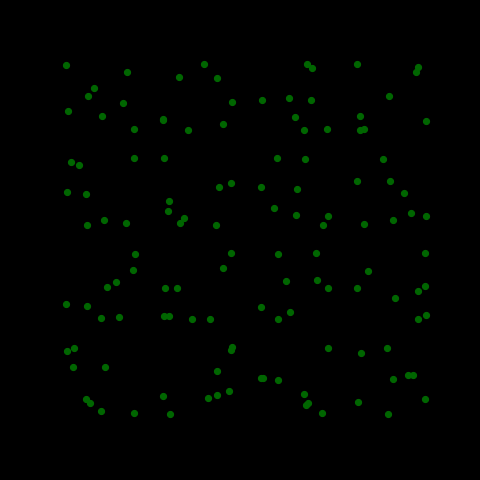
\includegraphics[scale=0.8]{Arboles8.png}
	\caption{Árboles maximales escogidos aleatoriamente con distribución uniforme entre todos los posibles en una gráfica completa de $8$ vértices}
	\label{fig:Arboles8}
\end{figure}

Llamaremos \textit{tiempo de cubrimiento} $C_{v}$ a el primer momento en que la partícula visitó todos los vértices de la gráfica empezando en $v$. Claramente el tiempo esperado de ejecución del algoritmo por árbol es igual a $\E(C_{s})$. Se sabe que para cada gráfica conexa $\E(C_{v}) = O(n^{3})$, sin embargo en \cite{BS89} se prueba que si la matriz de transición de una caminata aleatoria tiene el segundo eigenvalor más grande acotado lejos de 1, entonces el tiempo de cubrimiento esperado es sólo $O(n\cdot log(n))$. Esta condición la satisfacen la mayoría de las gráficas en el modelo $\G(n,p)$ para cada $p > \frac{c\cdot log(n)}{n}$ en particular $p=\frac{1}{2}$ y para casi todas la gráfica d-regulares \cite{BS87}, \cite{FKS89}. En la figura \ref{fig:tiemposGEN} se muestran los resultados del tiempo de ejecución para el algoritmo implementado en Python.

\begin{figure}[h!]
	\centering
	\includegraphics[scale=0.8]{tiemposGEN.png}
	\caption{Tiempos de ejecución en segundos del algoritmo generate variando el tamaño del árbol. Se presenta la escala norma y la logarítmica}
	\label{fig:tiemposGEN}
\end{figure}
